% !TeX root = ../../../book.tex

\subsection{原像:定义与示例}

你可能会问:那反过来呢?我们能否取值域的一个子集,然后找出哪些定义域中的元素的输出落在该子集中?当然可以!接下来的定义将为这一概念提供一个术语,你会发现它与``像''的定义有很多相似之处。

\subsubsection*{定义}

\begin{definition}
    设 $A, B$ 为集合,$f:A \to B$ 为函数。设 $Y \subseteq B$。

    \dotuline{$Y$ 在函数 $f$ 下的原像} 写做 $PreIm_f(Y)$,定义为
    \[PreIm_f (Y) = \{a \in A \mid f(a) \in Y \}\]
    也就是说,$Y$ 在函数 $f$ 下的原像是所有能产生 $Y$ 中``输出''的``输入''的集合。

    (当函数明确且无歧义时,我们有时会将符号简写为 $PreIm(Y)$,并将其称为 ``$Y$ 的原像'',而不是``$Y$ 在函数 $f$ 下的原像''。)
\end{definition}

首先思考一下:什么是 $PreIm_f (B)$?这里 $B$ 是整个值域。

回顾一下定义:$PreIm_f (B)$ 是所有输入 (在 $A$ 中) 的集合,这些输入的输出``落''在 $B$ 上。由于 $f$ 是一个良好定义的函数,所以 $PreIm_f (B)$ 实际上就是整个 $A$。因此,我们通常只会关注 $Y \subset B$ 的情况,因为这些情况更有趣。

\subsubsection*{示例}

\begin{example}
    第一个例子沿用了我们在上一节中讨论图时定义的函数。我们会再次展示示意图,但不会重新定义函数的所有细节。(详细信息请参见示例 \ref{ex:example7.3.2}。)

    \begin{center}
        {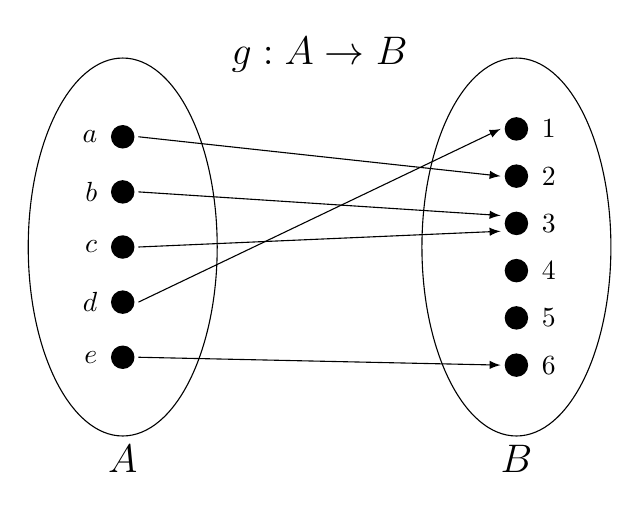
\begin{tikzpicture}[scale=1]
            \foreach \x in  {1,...,6}
            {
                \node at (5, -\x*0.6)[circle,fill,inner sep=3pt]{};
                \draw[shift={(5.2, -\x*0.6)}] node[right] {$\x$};
            }
            \draw (5,-2.1) ellipse (1.2 and 2.4);
    
            \foreach \x/\s in  {1/a,2/b,3/c,4/d,5/e}
            {
                \node at (0, -\x*0.7)[circle,fill,inner sep=3pt]{};
                \draw[shift={(-0.2, -\x*0.7)}] node[left] {$\s$};
            }
            \draw (0,-2.1) ellipse (1.2 and 2.4);
    
            \draw[-latex] (0.2,-0.7) -- (4.8,-1.2); 
            \draw[-latex] (0.2,-1.4) -- (4.8,-1.7); 
            \draw[-latex] (0.2,-2.1) -- (4.8,-1.9); 
            \draw[-latex] (0.2,-2.8) -- (4.8,-0.6); 
            \draw[-latex] (0.2,-3.5) -- (4.8,-3.6);
            
            \node[below] at (0, -4.5){\Large $A$};
            \node[below] at (5, -4.5){\Large $B$};
            \node[above] at (2.5, 0){\Large $g:A \to B$};
        \end{tikzpicture}}
    \end{center}

    定义 $Z_1 = \{1, 2, 3\}, Z_2 = \{2, 3, 4\}, Z_3 = \{4, 5, 6\}$。

    让我们识别并解释以下原像。

    \begin{enumerate}[label=(\arabic*)]
        \item $PreIm_g(\{1\}) = \{d\}$ \\
            因为 $g(d) = 1$ 且没有其他 $x \in A$ 满足 $g(x) = 1$。\\
            (注意,这里需要使用\emph{大括号}。``$PreIm_g(1)$'' 是没有意义的。)
        \item $PreIm_g(\{4\}) = \varnothing$ \\
            因为没有 $x \in A$ 满足 $g(x) = 4$。
        \item $PreIm_g(Z_1) = \{a, b, c, d\}$ \\
            因为 $g(a) = 2, g(b) = g(c) = 3, g(d) = 1$,但没有其他 $x \in A$ 满足 $g(x) \in Z_1$。
        \item $PreIm_g(Z_2) = \{a, b, c\}$ \\
            因为 $g(a) = 2, g(b) = g(c) = 3$,但没有其他 $x \in A$ 满足 $g(x) \in Z_2$。
        \item $PreIm_g(Z_3) = \{e\}$ \\
            因为 $g(e) = 6$,但没有其他 $x \in A$ 满足 $g(x) \in Z_3$。
        \item $PreImg(\{5\}) = \varnothing$ \\
            因为 $\forall x \in A \centerdot g(x) \ne 5$。
    \end{enumerate}
\end{example}

\begin{example}
    设函数 $f : \mathbb{R} \to \mathbb{R}$ 定义为 $\forall x \in \mathbb{R} \centerdot f(x) = x^2$。

    现在我们用这个函数来找几个原像。这次,我们希望你自己弄清楚为什么我们的结论是正确的,并尝试解释和证明它们。

    \begin{enumerate}[label=(\arabic*)]
        \item $PreIm_f (\{1\}) = \{-1, 1\}$
        \item $PreIm_f (\{y \in \mathbb{R} \mid y < 0\}) = \varnothing$
        \item $PreIm_f (\{y \in \mathbb{R} \mid y \ge 0\}) = \mathbb{R}$
        \item $PreIm_f (\{y \in \mathbb{R} \mid 0 < y < 1\}) = \{x \in \mathbb{R} \mid -1 < x < 1\}$
    \end{enumerate}
\end{example}